%%%%%%%%%%%%%%%%%%%%%%%%%%%%%%%%%%%%%%%%%
% Lachaise Assignment
% LaTeX Template
% Version 1.0 (26/6/2018)
%
% This template originates from:
% http://www.LaTeXTemplates.com
%
% Authors:
% Marion Lachaise & François Févotte
% Vel (vel@LaTeXTemplates.com)
%
% License:
% CC BY-NC-SA 3.0 (http://creativecommons.org/licenses/by-nc-sa/3.0/)
% 
%%%%%%%%%%%%%%%%%%%%%%%%%%%%%%%%%%%%%%%%%

%----------------------------------------------------------------------------------------
%	PACKAGES AND OTHER DOCUMENT CONFIGURATIONS
%----------------------------------------------------------------------------------------

\documentclass{article}

%%%%%%%%%%%%%%%%%%%%%%%%%%%%%%%%%%%%%%%%%
% Lachaise Assignment
% Structure Specification File
% Version 1.0 (26/6/2018)
%
% This template originates from:
% http://www.LaTeXTemplates.com
%
% Authors:
% Marion Lachaise & François Févotte
% Vel (vel@LaTeXTemplates.com)
%
% License:
% CC BY-NC-SA 3.0 (http://creativecommons.org/licenses/by-nc-sa/3.0/)
% 
%%%%%%%%%%%%%%%%%%%%%%%%%%%%%%%%%%%%%%%%%

%----------------------------------------------------------------------------------------
%	PACKAGES AND OTHER DOCUMENT CONFIGURATIONS
%----------------------------------------------------------------------------------------

\usepackage{keystroke} % https://ctan.crest.fr/tex-archive/macros/latex/contrib/keystroke/key-test.pdf

\usepackage{amsmath,amsfonts,stmaryrd,amssymb} % Math packages

\usepackage{minted} 

\usepackage{enumerate} % Custom item numbers for enumerations

\usepackage[ruled]{algorithm2e} % Algorithms

\usepackage[framemethod=tikz]{mdframed} % Allows defining custom boxed/framed environments

\usepackage{listings} % File listings, with syntax highlighting
\lstset{
	basicstyle=\ttfamily, % Typeset listings in monospace font
}

\usepackage{dirtree}

\usepackage{xcolor}

\usepackage{graphicx}

\usepackage{hyperref}
%----------------------------------------------------------------------------------------
%	DOCUMENT MARGINS
%----------------------------------------------------------------------------------------

\usepackage{geometry} % Required for adjusting page dimensions and margins

\geometry{
	paper=a4paper, % Paper size, change to letterpaper for US letter size
	top=2.5cm, % Top margin
	bottom=3cm, % Bottom margin
	left=2.5cm, % Left margin
	right=2.5cm, % Right margin
	headheight=14pt, % Header height
	footskip=1.5cm, % Space from the bottom margin to the baseline of the footer
	headsep=1.2cm, % Space from the top margin to the baseline of the header
	%showframe, % Uncomment to show how the type block is set on the page
}

%----------------------------------------------------------------------------------------
%	FONTS
%----------------------------------------------------------------------------------------

\usepackage[utf8]{inputenc} % Required for inputting international characters
\usepackage[T1]{fontenc} % Output font encoding for international characters

\usepackage{XCharter} % Use the XCharter fonts

%----------------------------------------------------------------------------------------
%	COMMAND LINE ENVIRONMENT
%----------------------------------------------------------------------------------------

% Usage:
% \begin{commandline}
%	\begin{verbatim}
%		$ ls
%		
%		Applications	Desktop	...
%	\end{verbatim}
% \end{commandline}

\mdfdefinestyle{commandline}{
	leftmargin=10pt,
	rightmargin=10pt,
	innerleftmargin=15pt,
	middlelinecolor=black!50!white,
	middlelinewidth=2pt,
	frametitlerule=false,
	backgroundcolor=black!5!white,
	frametitle={Command Line},
	frametitlefont={\normalfont\sffamily\color{white}\hspace{-1em}},
	frametitlebackgroundcolor=black!50!white,
	nobreak,
}

% Define a custom environment for command-line snapshots
\newenvironment{commandline}{
	\medskip
	\begin{mdframed}[style=commandline]
}{
	\end{mdframed}
	\medskip
}

%----------------------------------------------------------------------------------------
%	FILE CONTENTS ENVIRONMENT
%----------------------------------------------------------------------------------------

% Usage:
% \begin{file}[optional filename, defaults to "File"]
%	File contents, for example, with a listings environment
% \end{file}

\mdfdefinestyle{file}{
	innertopmargin=1.6\baselineskip,
	innerbottommargin=0.8\baselineskip,
	topline=false, bottomline=false,
	leftline=false, rightline=false,
	leftmargin=2cm,
	rightmargin=2cm,
	singleextra={%
		\draw[fill=black!10!white](P)++(0,-1.2em)rectangle(P-|O);
		\node[anchor=north west]
		at(P-|O){\ttfamily\mdfilename};
		%
		\def\l{3em}
		\draw(O-|P)++(-\l,0)--++(\l,\l)--(P)--(P-|O)--(O)--cycle;
		\draw(O-|P)++(-\l,0)--++(0,\l)--++(\l,0);
	},
	nobreak,
}

% Define a custom environment for file contents
\newenvironment{file}[1][File]{ % Set the default filename to "File"
	\medskip
	\newcommand{\mdfilename}{#1}
	\begin{mdframed}[style=file]
}{
	\end{mdframed}
	\medskip
}

%----------------------------------------------------------------------------------------
%	NUMBERED QUESTIONS ENVIRONMENT
%----------------------------------------------------------------------------------------

% Usage:
% \begin{question}[optional title]
%	Question contents
% \end{question}

\mdfdefinestyle{question}{
	innertopmargin=1.2\baselineskip,
	innerbottommargin=0.8\baselineskip,
	roundcorner=5pt,
	nobreak,
	singleextra={%
		\draw(P-|O)node[xshift=1em,anchor=west,fill=white,draw,rounded corners=5pt]{%
		Question \theQuestion\questionTitle};
	},
}

\newcounter{Question} % Stores the current question number that gets iterated with each new question

% Define a custom environment for numbered questions
\newenvironment{question}[1][\unskip]{
	\bigskip
	\stepcounter{Question}
	\newcommand{\questionTitle}{~#1}
	\begin{mdframed}[style=question]
}{
	\end{mdframed}
	\medskip
}

%----------------------------------------------------------------------------------------
%	WARNING TEXT ENVIRONMENT
%----------------------------------------------------------------------------------------

% Usage:
% \begin{warn}[optional title, defaults to "Warning:"]
%	Contents
% \end{warn}

\mdfdefinestyle{warning}{
	topline=false, bottomline=false,
	leftline=false, rightline=false,
	nobreak,
	singleextra={%
		\draw(P-|O)++(-0.5em,0)node(tmp1){};
		\draw(P-|O)++(0.5em,0)node(tmp2){};
		\fill[black,rotate around={45:(P-|O)}](tmp1)rectangle(tmp2);
		\node at(P-|O){\color{white}\scriptsize\bf !};
		\draw[very thick](P-|O)++(0,-1em)--(O);%--(O-|P);
	}
}

% Define a custom environment for warning text
\newenvironment{warn}[1][Warning:]{ % Set the default warning to "Warning:"
	\medskip
	\begin{mdframed}[style=warning]
		\noindent{\textbf{#1}}
}{
	\end{mdframed}
}

%----------------------------------------------------------------------------------------
%	INFORMATION ENVIRONMENT
%----------------------------------------------------------------------------------------

% Usage:
% \begin{info}[optional title, defaults to "Info:"]
% 	contents
% 	\end{info}

\mdfdefinestyle{info}{%
	topline=false, bottomline=false,
	leftline=false, rightline=false,
	nobreak,
	singleextra={%
		\fill[black](P-|O)circle[radius=0.4em];
		\node at(P-|O){\color{white}\scriptsize\bf i};
		\draw[very thick](P-|O)++(0,-0.8em)--(O);%--(O-|P);
	}
}

% Define a custom environment for information
\newenvironment{info}[1][Info:]{ % Set the default title to "Info:"
	\medskip
	\begin{mdframed}[style=info]
		\noindent{\textbf{#1}}
}{
	\end{mdframed}
}


%----------------------------------------------------------------------------------------
%	EQUATION
%----------------------------------------------------------------------------------------

\newcommand{\equabezier}{
	\begin{displaymath}
		P(t) = P_0(1-t)^3+3P_1t(1-t)^2+3P_2t^2(1-t)+P_3t^3	
	\end{displaymath}
} % Include the file specifying the document structure and custom commands

%----------------------------------------------------------------------------------------
%	ASSIGNMENT INFORMATION
%----------------------------------------------------------------------------------------

\title{Système et réseaux : rapport} % Title of the assignment
\author{Valentin VERSTRACTE \& Evan PETIT}

\date{L3 --- \today} % University, school and/or department name(s) and a date



%----------------------------------------------------------------------------------------

\begin{document}

\maketitle % Print the title

\bigskip
\bigskip
\renewcommand{\contentsname}{Table des matières}
\tableofcontents

\bigskip
\bigskip

\section*{Rappel des règles}
\addcontentsline{toc}{section}{\protect\numberline{}Rappel des règles}%
Le jeu se joue en plusieurs manches. Lors de la première manche,
chaque joueur reçoit une carte dont il prend connaissance. Ces cartes représentent les chiffres de 1 à 100. Le jeu est coopératif, il suffit de jouer les cartes par ordre croissant. De la plus petite à la plus grosse. C’est vraiment idiot. Mais voilà, le truc c’est que personne ne doit se parler, ni se faire des signes. Il n’y a donc pas d’ordre de jeu. Celle ou celui qui pense avoir la plus petite carte la pose. La ou le suivant qui pense avoir la plus petite suivante la pose et ainsi de suite

\section*{Introduction}
\addcontentsline{toc}{section}{\protect\numberline{}Introduction}%
L'application est découpé en 3 programmes shell. GestionJeu, JoueurHumain, JoueurRobot. Chacun d'eux utilisent des terminaux pour afficher l'état du jeu ou demander des entrées. Nous allons tout d'abord présenter comment les scripts communiquent et ensuite la structure.

\newpage
%----------------------------------------------------------------------------------------
%	Introduction
%----------------------------------------------------------------------------------------


\section{La communication}

Il existe dans ce projet plusieurs types de communications. On utilise les pipes pour communiquer des données et notifier des actions et les fichiers tmp pour synchroniser des données entre les shell et subshell  

\subsection{Les pipes : une micro API}

Chaque terminaux utilisent constamment des pipes pour recevoir ou envoyer des données / actions. Il a été choisit de construire une micro API pour faciliter cette communication. On envoie un message dans les pipes constituer de la forme suivante :
\begin{center}
[n°action];[message]
\end{center}
Le ";" permet de facilité la séparation et récupération du n°action et du message. Voici les n°action que l'on peut trouver:
\begin{itemize}
	\item N°1 décrit que la carte trouvée était la bonne.\newline Le message sera du type : \textit{Bravo, une carte a été trouvée, voici les cartes trouvées : (1 2 )}
	\item N°2 décrit que la carte trouvée était mauvaise.\newline Le message sera du type : \textit{Perdu, la carte 2 n'était pas la bonne, la bonne était : 1. On recommence !}  
	\item N°3 décrit que le tour est terminé, on passe au suivant.\newline Le message sera du type : \textit{Félicitations, le tour n°'2 est terminé, on passe au tour suivant} 
	\item N°4 décrit que le jeu est terminé, on passe au suivant.\newline Le message sera du type : \textit{Félicitations, le jeu est terminé}
	\item N°5 décrit que le joueur a reçu toutes ses cartes dans son fichier tmp     
	\item N°9 est spécifique au robot. Il répond à un problème technique. Brièvement à chaque fois qu'une carte est jouer le robot s'envoie à lui-même le message "9;distance" au bout d'un certain temps. "distance" étant la distance entre sa carte la plus faible et la dernière carte jouée. Comme ça si une nouvelle carte est jouée entre-temps, la distance change et on laisse au joueur le temps de réévaluer la situation.
	
\begin{figure}[!htb]
	\centering
    	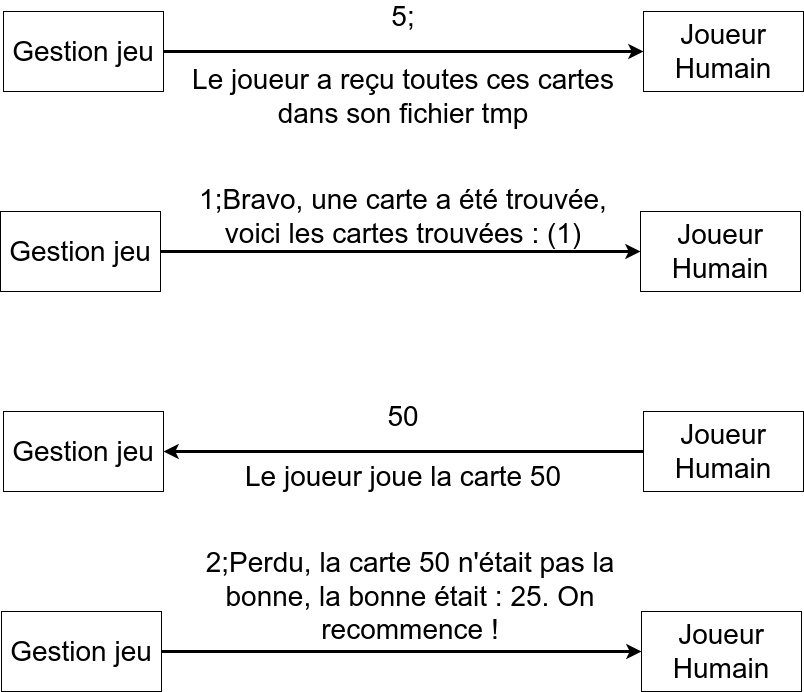
\includegraphics[height=8cm]{./assets/pipe_com.png}
    	\caption{
	    	Exemple d'une communication avec la micro API
    	}
    	\label{fig:pipe}
\end{figure}

On remarquera qu'il suffit d'envoyer un chiffre à gestion jeu pour qu'il soit interprété comme une carte jouée. Si l'application était beaucoup plus importante, cela pourrait représenter une faille de sécurité importante. 
  
\end{itemize}

\newpage
\subsection{Les fichiers tmp}
Les fichiers tmp sont présents pour résoudre le problème de synchronisation des variables entre le shell et le subshell (problème dû aux commandes bloquantes). Chaque ligne du fichier tmp représente une carte. On lit toutes les lignes pour savoir les cartes du joueur. Ainsi, pour transmettre des cartes, gestion jeu écrit dans le fichier tmp et envoie un message à travers les pipes pour décrire quand il a finit. Quand le joueur joue une carte, on réécrit toutes les cartes ligne à ligne dans le fichier sans celle jouée.


\section{Structure générale de l'application}

\subsection{Gestion Jeu}
\subsubsection{L'initialisation}

Une première phase de l'initialisation définit le nombre de joueurs. Elle le fait en demandant le nombre de joueurs humains puis le nombre de joueurs robots. On lance en conséquence les scripts nécessaires au travers d'un terminal xTerm. Chaque joueur humain obtient un terminal au travers du quel il peut interagir.
\newline
\newline
Une deuxième phase de l'initialisation s'occupe de chercher le nombre maximum de tour / carte maximum que l'on peut distribuer. Il s'agit d'un petit algorithme qui incrémente une variable en fonction d'une condition. Cette condition est la suivante : si la variable multipliée par le nombre de joueurs est inférieure à 100, alors on incrémente. On continue jusqu'à que la multiplication soit supérieure à 100. On en déduit à la fin le nombre maximum de tour.
\newline
\newline
La troisième phase de l'initialisation appelle la fonction qui gère les cartes. Nous allons décrire cette fonction dans la sous-section suivante puisqu'elle est appelée à différents moments de la partie.  

\subsubsection{La gestion des cartes}

La gestion des cartes a trois objectifs :

\begin{itemize}
	\item Mélanger aléatoirement les cartes
	\item Distribuer aux joueurs les cartes de 0 à N ( N = indice du rond multiplier par le nombre de joueur )
	\item Trier les cartes distribuer pour savoir dans quel ordre elles doivent être jouer
\end{itemize}

Ces trois objectifs devant être atteints de manière récurrente dans le code, ils sont contenus dans une fonction. Cette fonction est appelée après chaque ronde, à chaque fois qu'une mauvaise carte est jouée et lors de l'initialisation. 
\newline
\newline
Le troisième objectif est motivé par une idée simple : on souhaite juste savoir la carte qui doit être jouée sans savoir quel joueur doit la jouer. 

\subsubsection{La gestion du jeu}

À partir de l'API nous pouvons savoir une chose importante : 
une carte a été jouer et on connaît son nombre. C'est ici que tout prend son importance car nous allons effectuer en conséquence des traitements à partir de cette action.\newline
On regarde tout d'abord si la carte jouée est la carte qui devait être jouer (merci l'objectif 3 de la gestion de cartes). Si ce n'est pas le cas, on notifie les joueurs que la carte tirée est mauvaise et on redistribue des cartes (fonction gestion des cartes) et le tour recommence. Sinon, on notifie tous les joueurs de la carte trouver. On regarde ensuite si il s'agissait de la dernière carte du tour. Si c'est le cas et qu'il reste un tour, on passe au tour suivant en redistribuant des cartes. 

\subsection{Joueur Humain}
Le comportement du script de joueur humain est scindée en deux grandes parties. La première s'occupe de la réception des communications avec gestion jeu et de l'affichage. La deuxième de l'entrée utilisateur et de l'envoi de la carte jouée. Cette structure de code n'est pas venu naturellement. Elle répond à problème technique : chaque partie utilise une commande bloquante. 

\subsubsection{Le problème des commandes bloquantes}
On se retrouve avec deux commandes bloquantes. Une première essaye de lire les pipes, une deuxième essaye de lire l'entrée utilisateur. Pour résoudre ce problème nous avons choisi la solution suivante : l'entrée utilisateur sera lue par un subshell et les pipes seront lues à partir du shell. Un deuxième problème technique est alors apparu. Les variables entre le shell et le subshell ne sont pas synchronisées. Ceci représente une difficulté puisque nous avons besoin de savoir les cartes reçues depuis les pipes dans l'entrée utilisateur (pour savoir si l'utilisateur peut bien jouer cette carte). Cette difficulté a été résolu a l'aide des fichiers TMP.

\subsubsection{Réception des communications(API) / affichage}
La partie centrée sur la réception des communications et l'affichage lit constamment les pipes. En fonction du message reçu, une action en découle. Il peut très bien s'agir de lancer le subshell pour lire les entrées utilisateur ou afficher les informations reçues

\subsubsection{L'entrée utilisateur}
La partie centrée sur l'entrée utilisateur n'est pas très compliquée. Elle lit tout le temps le terminal. On est alors obligé de trier l'affichage et l'entrée utilisateur. Comme on souhaite lire la carte que l'utilisateur souhaite jouer et que l'affichage n'est jamais juste un chiffre on regarde si la lecture est un chiffre. Si c'est le cas on récupère les cartes de l'utilisateur dans son fichier tmp associé et on regarde si la carte voulant être jouer existe. Si c'est le cas, on la retire du fichier et on envoie la carte jouer à gestion jeu. 

\begin{figure}[!htb]
	\centering
    	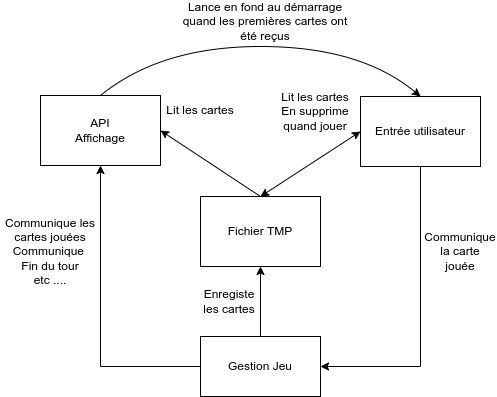
\includegraphics[height=10cm]{./assets/JoueurHumain.png}
    	\caption{Illustration / cycle de vie de joueur humain}
\end{figure}

\newpage

\subsection{Joueur robot}
Le premier réflexe a été de copier coller le code du joueur humain et de remplacer les entrées utilisateurs par une stratégie robot. 

\subsubsection{La stratégie}
Il a été difficile d'établir une stratégie pour le robot. Le problème a donc été décalé et on se repose sur le joueur. L'idée est simple. Quand le joueur estime que ce n'est pas son tour, il va laisser jouer. Ainsi, au bout d'un certain temps, le robot joue sa carte la plus faible. Malgré des faiblesses cette stratégie reste très forte car repose sur l'intelligence du joueur humain. 

\subsubsection{Réception des communications(API) / affichage}
La réception des communications reste le même principe que pour le joueur humain. Il existe cependant une exception qui est la réception de la distance comme expliquer dans la figure \ref{fig:pipe}. Elle permet de savoir si le robot doit jouer sa carte la plus faible ou non. 
%----------------------------------------------------------------------------------------

\end{document}
